\chapter{Predictive Selection and Arithmetic Certification}\label{ch:select}

Chapter~\ref{ch:schedule} proved that one prime survives. This chapter answers the next question: \emph{which one}, from finite arithmetic data. Three results do this. The carry-level predictor (Theorem~\ref{thm:predictor}) computes the next carry exactly; the minimax theorem (Theorem~\ref{thm:minimax}) shows that, in a system of independent odometers, the survivor is the prime with the smallest worst-case carry whatever the starting phases; and the static certificate (Theorem~\ref{thm:certificate}) turns this into a finite residue test at a single reset state, which certifies the whole infinite future.

\begin{remark}[Hypotheses of certification]\label{rem:certscope}
Static certification is proved for \emph{prime} \(g\), or more generally for \(g\) with no prime factor \(\le m^2\) (hypothesis (S5) below). It does not extend to composite or even \(g\): for the persistent values \(g=15,39,51,57,68,87\), every reset state fails (S5) (Theorem~\ref{thm:consequences}). The theorems below state this hypothesis where it is used.
\end{remark}

\section{The exact carry-level predictor}

A \emph{reset state} is a state with \(\gamma=1\). For \(M\ge2\) and a state \(E\), \(M=\prod p^{j_p}\) is \emph{available} if there is \(a\in\prod_{q\nmid M}\{q^i:0\le i\le e_q\}\) with \(\prod_{p\mid M}p^{e_p+j_p}\cdot a\equiv1\ (\mathrm{mod}\ g)\).

\begin{theorem}[Exact carry-level predictor]\rec{F.T67}\scope{C}\label{thm:predictor}
From a reset state \(E\) (exact \(G=g\)) of a persistent orbit, the next carry is
\[
M^\ast=\min\{M\ge2:\ M\text{ available at }E\}.
\]
The next state is \(E'=E\) with \(e_p\) increased by \(\vv_p(M^\ast)\) for every \(p\mid M^\ast\); \(\gamma'=1\) again, and the carry occupies the \(\gamma\)-steps \(1,2,\dots,M^{\ast2}-1\) (\(w=2,\dots,M^{\ast2}\)). The orbit remains persistent through this carry iff \(M^{\ast2}<g\) when \(g\) is an odd prime (in general iff in addition \(\gcd(g,w)=1\) for all \(w\le M^{\ast2}\), e.g. when every prime factor of \(g\) exceeds \(M^{\ast2}\)). Consequently every state after the first reset state is a reset state, and the orbit is the iteration \(E\mapsto E'\) of this map: there is no partial absorption after the first reset.
\end{theorem}
\begin{proof}
By Theorem~\ref{thm:absorb} a divisor \(d\equiv1\ (\mathrm{mod}\ g)\) is available at the step \(w\) iff \(M(d)^2\mid w\), with \(M(d)\) the new part. Write \(d=\prod_{p\mid M}p^{e_p+j_p}\cdot a\) with \(M=M(d)\) and \(a\) built from primes \(q\nmid M\) with \(\vv_q(a)\le e_q\): this is exactly the statement ``\(M\) is available''. The first \(w\ge2\) for which some \(d\) has \(M(d)>1\) and \(M(d)^2\mid w\) is \(w=M^{\ast2}\), \(M^\ast=\min M(d)\) (Theorem~\ref{thm:carrycomp}: from \(\gamma=1\) the plateau runs to \(w=M^{\ast2}\)). At \(w=M^{\ast2}\) the available new parts are those \(M(d)\) with \(M(d)\mid M^\ast\); by minimality only \(M(d)=M^\ast\), so \(r=\mathrm{lcm}=M^\ast\) and \(\gamma'=w/r^2=1\). For prime \(g\), all \(w\le M^{\ast2}\) are \(<g\) exactly when \(M^{\ast2}<g\); then \(h=1\) and persistence is automatic by Theorem~\ref{thm:onestep}.
\end{proof}

\section{The minimax selection theorem}

\emph{Setting (independent odometers).} Primes \(p_1<\dots<p_k\), each with a nonempty set \(\Abs_i\subseteq\Z/o_i\) and a state \(e_i\in\Z/o_i\). The pending carry is \(c_i(e_i)=p_i^{\mathrm{gap}_i(e_i)}\), \(\mathrm{gap}_i(e)=\min\{j\ge1:(e+j)\bmod o_i\in\Abs_i\}\); the smallest pending carry fires and \(e_i\leftarrow e_i+\mathrm{gap}_i(e_i)\). Let \(d_i\) be the largest cyclic gap of \(\Abs_i\) (differences of consecutive elements, with \(o_i+a_1-a_r\) for the wrap-around) and \(m_i=p_i^{d_i}\), the \emph{worst-case carry}.

\begin{theorem}[Minimax selection]\rec{F.T64}\scope{C}\label{thm:minimax}
\begin{enumerate}[label=(\roman*),nosep]
\item \(c_i(e)\le m_i\) for every phase \(e\).
\item Every walk, from every start phase, ends in a cycle in which exactly one prime fires, namely \(p_\ast=\arg\min_im_i\).
\item With a window (a pending carry \(\ge W\) is forbidden, i.e. the orbit leaves persistence), the system stays admissible forever iff \(m_{p_\ast}<W\); if \(m_{p_\ast}\ge W\), every walk exits in finite time.
\end{enumerate}
\end{theorem}
\begin{proof}
(i) The phase \(e\) lies in a cyclic interval between consecutive elements of \(\Abs_i\) (or is one of them); \(\mathrm{gap}(e)\) is the distance to the right end, hence at most the length of that interval, hence \(\le d_i\).
(ii) Some prime fires infinitely often (finitely many primes, one fires per step). Suppose \(r\) fires infinitely often and \(r\ne p_\ast\). The phase of \(r\) takes every value of \(\Abs_r\) cyclically, in particular the one before a gap of length \(d_r\), where its pending carry is \(m_r\). There \(r\) fires only if \(m_r<c_{p_\ast}(e_{p_\ast})\le m_{p_\ast}\) by (i). But \(m_r>m_{p_\ast}\) (the \(m_i\) of distinct primes are distinct, and \(p_\ast\) has the smallest). Contradiction; so only \(p_\ast\) fires infinitely often.
(iii) If \(m_{p_\ast}<W\), the smallest pending carry is \(\le c_{p_\ast}\le m_{p_\ast}<W\) at every step, so there is no exit. If \(m_{p_\ast}\ge W\), then \(p_\ast\) eventually sits in its worst-case phase, where the smallest pending carry is \(m_{p_\ast}\ge W\) (every competitor's pending carry is frozen above it): exit.
\end{proof}

This sharpens Theorem~\ref{thm:dominance}, which proved ``at most one'', to a non-iterative, phase-independent selection rule. It does not by itself apply to the collective map, because there the odometer tables depend on the actual state (Theorem~\ref{thm:certificate}).

\section{The quotient-residue formula}

\begin{theorem}[Quotient-residue formula]\rec{F.T65}\scope{C}\label{thm:quotient}
Let \(p\) be a prime with \(\gcd(p,g)=1\); \(H\le(\Z/g)^\times\) the subgroup generated by the residues of the \emph{saturated} other primes (\(e\ge o-1\)); \(F\) the set of residues of the divisors of the frozen (unsaturated or inert) other primes' part; \(t_p\) the order of \(pH\) in \((\Z/g)^\times/H\). Put
\[
S_p=\{r\bmod t_p:\ p^rf\in H\text{ for some }f\in F\}.
\]
Then
\[
\Abs_p=\{k\bmod o_p:\ k\bmod t_p\in S_p\},
\]
a union of residue classes modulo \(t_p\) (with \(t_p\mid o_p\)); the gaps of \(\Abs_p\) in \(\Z/o_p\) are the gaps of \(S_p\) in \(\Z/t_p\), so \(m_p=p^{\mathrm{maxgap}(S_p)}\) (cyclic maximum in \(\Z/t_p\)). For prime \(g\), \(t_p=o_p/\gcd(o_p,|H|)\).
\end{theorem}
\begin{proof}
\(\Abs_p=\{k:p^{-k}\in\mathcal A_{-p}\}\) with \(\mathcal A_{-p}=H\cdot F\) (each saturated prime contributes a whole cyclic subgroup, and their product is \(H\)). Now \(p^{-k}\in HF\) iff \(p^{-k}H=fH\) for some \(f\in F\), i.e. iff \(p^kf\in H\). This depends only on \(k\bmod t_p\) since \(p^{t_p}\in H\). For prime \(g\) the unit group is cyclic, \(|\langle p\rangle\cap H|=\gcd(o_p,|H|)\), so \(t_p=o_p/|\langle p\rangle\cap H|\).
\end{proof}

The formula replaces ``walk the odometer'' by a finite computation in a quotient group; it holds for composite \(g\) as well (there the quotient need not be cyclic and \(t_p\) is the plain order), and it generalises Theorem~\ref{thm:coprime} to any saturated background.

\section{The static certificate}

\begin{theorem}[Static survivor certificate]\rec{F.T66}\scope{C}\label{thm:certificate}
\emph{Hypotheses (finite data of one reset state \(E\)).} \(g\) is prime, or more generally \(g\) has no prime factor \(\le m^2\) \textup{(S5)}; \(G(x)=g\) exactly; \(E\) is a reset state (\(\gamma=1\)); a prime \(r\nmid g\) is saturated in \(E\) (\(e_r\ge o_r-1\)). Let \(\Abs_r\) be computed from the other primes' residue sets (Theorems~\ref{thm:odometer},~\ref{thm:quotient}), \(d_r\) its largest cyclic gap and \(m=r^{d_r}\).
\begin{itemize}[nosep]
\item[(S3)] \(m^2<g\);
\item[(S4)] no \(M\) with \(2\le M<m\) and \(\gcd(M,r)=1\) is available at \(E\);
\item[(S5)] no prime factor of \(g\) is \(\le m^2\).
\end{itemize}
\emph{Conclusion.} Under (S3)--(S5) the orbit from \(E\) is persistent forever and only \(r\) carries: the carries are \(r^j\) with \(j\) running cyclically through the gaps of \(\Abs_r\) (starting at the phase \(e_r\bmod o_r\)); the \(\gamma\)-period is \(\sum_i(r^{2j_i}-1)\) over one period \(s\) of \(\Abs_r\), \(\rho=r^s\), and \(x_{n+P}=r^{2s}x_n\) for all \(n\ge0\) (not only eventually). Conversely, for prime \(g\): if \(r\) is saturated, \(E\) is a reset state, and the orbit carries only \(r\) from \(E\) on and stays persistent, then (S3) and (S4) hold ((S5) is automatic for prime \(g>m^2\)).
\end{theorem}
\begin{proof}
\emph{Sufficiency.} Induction on carries. Let \(E\) be a reset state with (S3)--(S5) and \(r\) saturated, and let \(M^\ast\) be the smallest available \(M\) (Theorem~\ref{thm:predictor}).

(a) If \(M=r^as\) with \(a\ge1\), \(s>1\) coprime to \(r\) is available, then so is \(s\) alone: since \(r\) is saturated, choose \(i\in[0,o_r-1]\) with \(i\equiv e_r+a\ (\mathrm{mod}\ o_r)\); then \(i\le e_r\), and \(d'=d\,r^{i-e_r-a}\) is a smaller divisor \(\equiv d\equiv1\) with new part \(s\) (the argument of Theorem~\ref{thm:primepower}). So the smallest available \(M\) is either a pure power \(r^a\) or coprime to \(r\).

(b) By (S4) every coprime available \(M\) is \(\ge m\), and \(=m\) is impossible (\(m\) is a power of \(r\)); so every coprime available \(M\) exceeds \(m\).

(c) A pure power \(r^a\) is available iff \((e_r+a)\bmod o_r\in\Abs_r\) (Theorem~\ref{thm:odometer}); the smallest such \(a\) is the gap at the current phase, so \(r^a\le m\). Hence \(M^\ast=r^{\mathrm{gap}(\varphi)}\le m<\) every coprime available \(M\), and \(M^{\ast2}\le m^2<g\) by (S3), with \(\gcd(g,w)=1\) for all \(w\le M^{\ast2}\) by (S5). By Theorem~\ref{thm:predictor} the carry is \(r^{\mathrm{gap}}\), and the state after it, \(E'\), is \(E\) with \(e_r\) increased by the gap: again a reset state with \(r\) saturated and all other exponents unchanged. \(\Abs_r\) and the availability of coprime \(M\) do not change: the residue set of \(r\) among the divisors is the full subgroup \(\langle r\rangle\) (saturated) and every coprime \(M\) ignores the exponent of \(r\). So (S3)--(S5) hold at \(E'\) and the induction continues, the phase moving along the gaps of \(\Abs_r\). The periodicity statement is Theorem~\ref{thm:rho}.

\emph{Necessity (prime \(g\)).} If \(r\) carries forever, it visits the phase at which its pending carry is \(m\) (equality in Theorem~\ref{thm:minimax}(i): the phase before the largest gap), where \(M^\ast=m\). Any available coprime \(M\) would have to exceed \(m\) (it cannot equal a power of \(r\)), hence none is \(<m\): (S4). Persistence gives \(m^2<g\) (Theorem~\ref{thm:window}: the carry \(m\) passes through \(w=g\) otherwise): (S3). For prime \(g\), (S5) is then automatic.
\end{proof}

\begin{proposition}[Unsaturated extension and uniqueness]\scope{C}\label{prop:T66p}
(Part of the source record \texttt{F.T66}, where it is stated as T66$'$ and the uniqueness clause.)
(a) If \(e_r<o_r-1\), apply Theorem~\ref{thm:predictor} to the phases \(e_r,e_r+\mathrm{gap},\dots\) until \(e_r\ge o_r-1\) (at most \(o_r-1\) carries; only \(r\)'s exponent moves as long as each next carry equals the predicted power of \(r\)), then Theorem~\ref{thm:certificate}: a finite check over \(r\)-carries only. (b) At most one prime is certified from a state.
\end{proposition}
\begin{proof}
(a) is the concatenation of the two finite procedures. (b) If \(r_1\ne r_2\) were both certified, (S4) for \(r_1\) gives \(c_{r_2}>m_{r_1}\ge c_{r_1}\), and (S4) for \(r_2\) gives \(c_{r_1}>m_{r_2}\ge c_{r_2}\); so \(c_{r_2}>c_{r_1}>c_{r_2}\), a contradiction.
\end{proof}

\emph{What the certificate does not claim.} The competitor condition (S4) concerns the \emph{actual} state: the hypothetical tables of Theorem~\ref{thm:minimax} for other primes are not used, because a competitor's \(\Abs\) depends on \(r\) being saturated. Seeds that are not reset states (\(\gamma_0>1\)) and the moduli \(g\) discussed in Remark~\ref{rem:certscope} lie outside the theorem; \(\gamma_0>1\) is handled by the transient bounds of Chapter~\ref{ch:bounds}.

\begin{example}[A certified state at \(g=127\)]\label{ex:cert127}
At the reset state \(E=\{2{:}6,\,3{:}6,\,11{:}2,\,41{:}6\}\) with \(g=127\) (checked by normalisation to have \(\gamma=1\)), the pending carries are \(c_2=4\), \(c_3=9\), \(c_5=5\), \(c_7=7\); the prime \(2\) is saturated (\(o_2=7\), \(\Abs=\{0,2,3,4,6\}\), largest gap 2, \(m=4\)); \(m^2=16<127\), and \(127\) is prime (S5); no coprime \(M\in\{3\}\) with \(M<4\) is available. So (S3)--(S5) hold and the prime \(2\) carries forever, with \(P_\gamma\) given by Theorem~\ref{thm:rho}. Figure~\ref{fig:selection} shows the pending carries against the worst-case bar \(m\) and the availability of each candidate \(M\).
\end{example}

\begin{figure}[t]
\centering
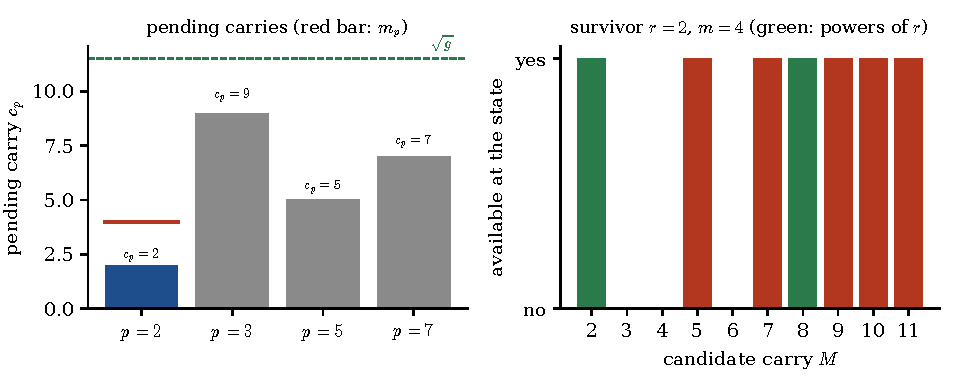
\includegraphics[width=0.97\linewidth]{figs/fig_selection.pdf}
\caption{A statically certified reset state at \(g=127\) (Example~\ref{ex:cert127}). Left: pending carries \(c_p\); the red bar marks the worst-case carry \(m_p\) of the saturated prime. Right: availability of each candidate carry \(M\le\sqrt g\) at the state; green bars are the powers of the survivor \(r=2\). No \(M<m=4\) coprime to \(2\) is available, which is hypothesis (S4); \(m^2=16<127\), which is (S3).}\label{fig:selection}
\end{figure}

\section{Consequences of certification}

\begin{theorem}[Consequences of static certification]\rec{F.T68}\scope{C}\label{thm:consequences}
\begin{enumerate}[label=(\alph*),nosep]
\item \emph{For prime \(g\):} every persistent orbit reaches a statically certified reset state (after its eventual regime is entered, Theorems~\ref{thm:closure},~\ref{thm:dominance}; every eventual reset state satisfies (S3)--(S5) for the active prime, by the necessity part of Theorem~\ref{thm:certificate}). So ``which prime survives'' is decided by a finite residue test at that state. \emph{For composite or even \(g\) this is not asserted:} for \(g=15,39,51,57,68,87\) every tested reset state fails (S5).
\item From a certified state the complete future is a function of finite data: the carry word (gaps of \(\Abs_r\) from the current phase), the \(\gamma\)-period \(\sum(r^{2j}-1)\), \(\rho=r^s\), and the window margin \(m^2<g\).
\item \(g\) alone does not determine the survivor; the pair \((g,\text{background }E)\) does. For \(g=31\) there are orbits with survivor \(2\) and orbits with survivor \(5\).
\end{enumerate}
\end{theorem}
\begin{proof}
(a) For prime \(g\) every eventual reset state has an active saturated prime \(r\) that carries forever from it and keeps the orbit persistent (Theorems~\ref{thm:closure},~\ref{thm:dominance}); the converse direction of Theorem~\ref{thm:certificate} then gives (S3), (S4), and (S5) is automatic. (b) is the conclusion of Theorem~\ref{thm:certificate}. (c) For \(g=31\): the reset state \(L_0=2^5\cdot101^2\) (so \(E_0=\{2{:}5,\,101{:}2\}\)) has survivor \(2\), with carries \(2^2,2^2,2^1\), \(P_\gamma=33\) and \(\rho=32\) (Example~\ref{ex:g31}); the template state of Theorem~\ref{thm:qcarry} with \(q=5\) has survivor \(5\), with \(P=24\), \(\rho=5\). Both are verified by direct iteration of \(C\) and by class closure (Theorem~\ref{thm:closure}).
\end{proof}

\begin{remark}[Scope statement]\label{rem:T73a}
The general phrasing ``every persistent orbit reaches a statically certified reset state'' is a theorem for prime \(g\) (Theorem~\ref{thm:consequences}(a)); for composite or even \(g\) the hypothesis (S5) fails at every reset state of the six cycles \(g=15,39,51,57,68,87\), so no certified state is available there (the registered correction is Theorem~\ref{thm:T73}), although each of these orbits still has exactly one active prime (Theorem~\ref{thm:dominance}) and an exact scaling law (Theorem~\ref{thm:rho}). Closing this gap is Open Problem~\ref{op:composite}.
\end{remark}
